\section{Higgs reconstruction}
\label{sec:ewk:higgsreco}

A key ingredient of the analysis is the reconstruction of the two Higgs bosons form the decay of the Higgsinos.
Since this analysis targets events where both Higgs bosons decay to a $b\bar{b}$ pair, the reconstruction starts 
from four jets, which are chosen according to an ordering criterion that favors b-tagged jets over non-tagged jets,
and then orders based on \pt. Practically, this results in the following criteria:
\begin{itemize}
\item If there are exactly four b-tagged jets in the event, those are used.
\item If there are more than four b-tagged jets, the selected ones are the four b-tagged jest with highest \pt.
\item If there are less than four b-tagged jets, the selected ones are the b-tagged ones and the non-tagged ones with highest \pt.
\end{itemize} 

Once the four jets have been selected, they are grouped in two pairs, each one constituting a candidate Higgs bosons. 
Different algorithms to pair the jets have been tested, and the chosen one is based on minimizing the angular separation 
between the two jets associated to the same Higgs boson candidate. 
In particular, the permutation chosen is the one that minimizes:
\begin{equation}
\dRmax = \mathrm{max}(\Delta R(h_1), \Delta R(h_2)) \; ,
\end{equation}

\noindent where $\Delta R(h)$ is the distance in the $\eta-\phi$ space between the two jest from the same candidate.
This choice has a good efficiency in reconstructing the Higgs bosons in the signal, 
and at the same time avoids creating artificial peaks in the background in correspondence of the Higgs boson mass. 

\section{Kinematic variables specific to this analysis}

Beside the variables described in Section \ref{sec:common_variables}, a few other discriminating variables particularly 
effective for this signal model are described in this section.

\subsubsection*{Candidate Higgs bosons}

The invariant mass of the two Higgs boson candidates built following the procedure outlined in Section \ref{sec:ewk:higgsreco} 
are used as discriminating variable. In particular, we refer to m($h_1$) and m($h_2$) respectively for the mass of the Higgs candidate with 
the leading and sub-leading mass.

The variable \dRmax, defined in the previous section, is used to choose the pairing of the jets while reconstructing 
the Higgs boson candidates but also as a discriminating variable to separate signal and background. 

\subsubsection*{Modified effective mass}

In the signal model, only four jets come from the hard scattering process, and are therefore expected to be more energetic than the 
remaining jets in the event. Therefore the \meff definition is modified to include only the jets that are selected 
as originating from a Higgs boson; the modified definition is therefore:
\begin{equation}
\meffb = \sum_{i=1,..,4} {\pt}^{j_i} + \met
\end{equation}
\noindent where the sum runs over the jets selected according to the ordering procedure presented in Section \ref{sec:ewk:higgsreco}. 


\section{Discriminating variables}

In this section we show how the variables defined in Section \ref{sec:common_variables} and the ones related
to the Higgs boson reconstruction (\dRmax defined in the previous section, and the mass of the reconstructed Higgs boson candidates)
allow to identify a region of the phase space that is enriched in signal events. 
This study is performed after selecting events with high \met ($> 200$ GeV), at least four signal jets and, least three b-tagged jets, zero signal leptons and \dphimin $>0.4$.
with at least one signal lepton.

Figure \ref{ffig:ewk:sig:1} shows the distribution of the main kinematic variables for 
the sum of the \gls{sm} backgrounds and for selected signal samples after these selections.
Figures \ref{fig:ewk:sig:mass_h1_min_dR} and \ref{fig:ewk:sig:mass_h2_min_dR} show the distribution of the mass of the Higgs 
candidate with the leading and sub-leading mass respectively. We can see how the distribution peaks at values around the Higgs mass for 
signals, while it is flatter for background. 
The distribution of \dRmax is shown in Figure \ref{fig:ewk:sig:dRmax_dR}. This variable assumes in general a lower value for 
signal events, in particular for the high-mass signals, where the Higgs bosons are produced with higher \pt and thus have 
more collimated decay products. Signal events tend also to have a lower number of signal jets, as can be observed in Figure 
\ref{fig:ewk:sig:jets_n}, and they occupy mostly the bins with three and four b-jets in the 
distribution of \nbjet (Figure \ref{fig:ewk:sig:bjets_n}). 
The \met distribution, shown in Figure \ref{fig:ewk:sig:met}, displays the expected features: while signals with low-mass Higgsinos 
have low \met values, the distribution tends to assume increasingly high values with the increase of the Higgsino mass. 
A similar feature is shown in Figures \ref{fig:ewk:sig:meff_4bj} and \ref{fig:ewk:sig:mTb_min} for the \meffb and \mtb distributions respectively: 
the higher the Higgsino mass in the signal, the more signal events differ form background events. 
While on the one hand this makes it easier to separate them from the \gls{sm} background, on the other hand the increase in signal mass 
implies a decrease in production cross section, which will be the limiting factor in sensitivity to high-mass signals. 

\begin{figure*}[htbp]
\centering 
\subfigure[m($h_1$)]{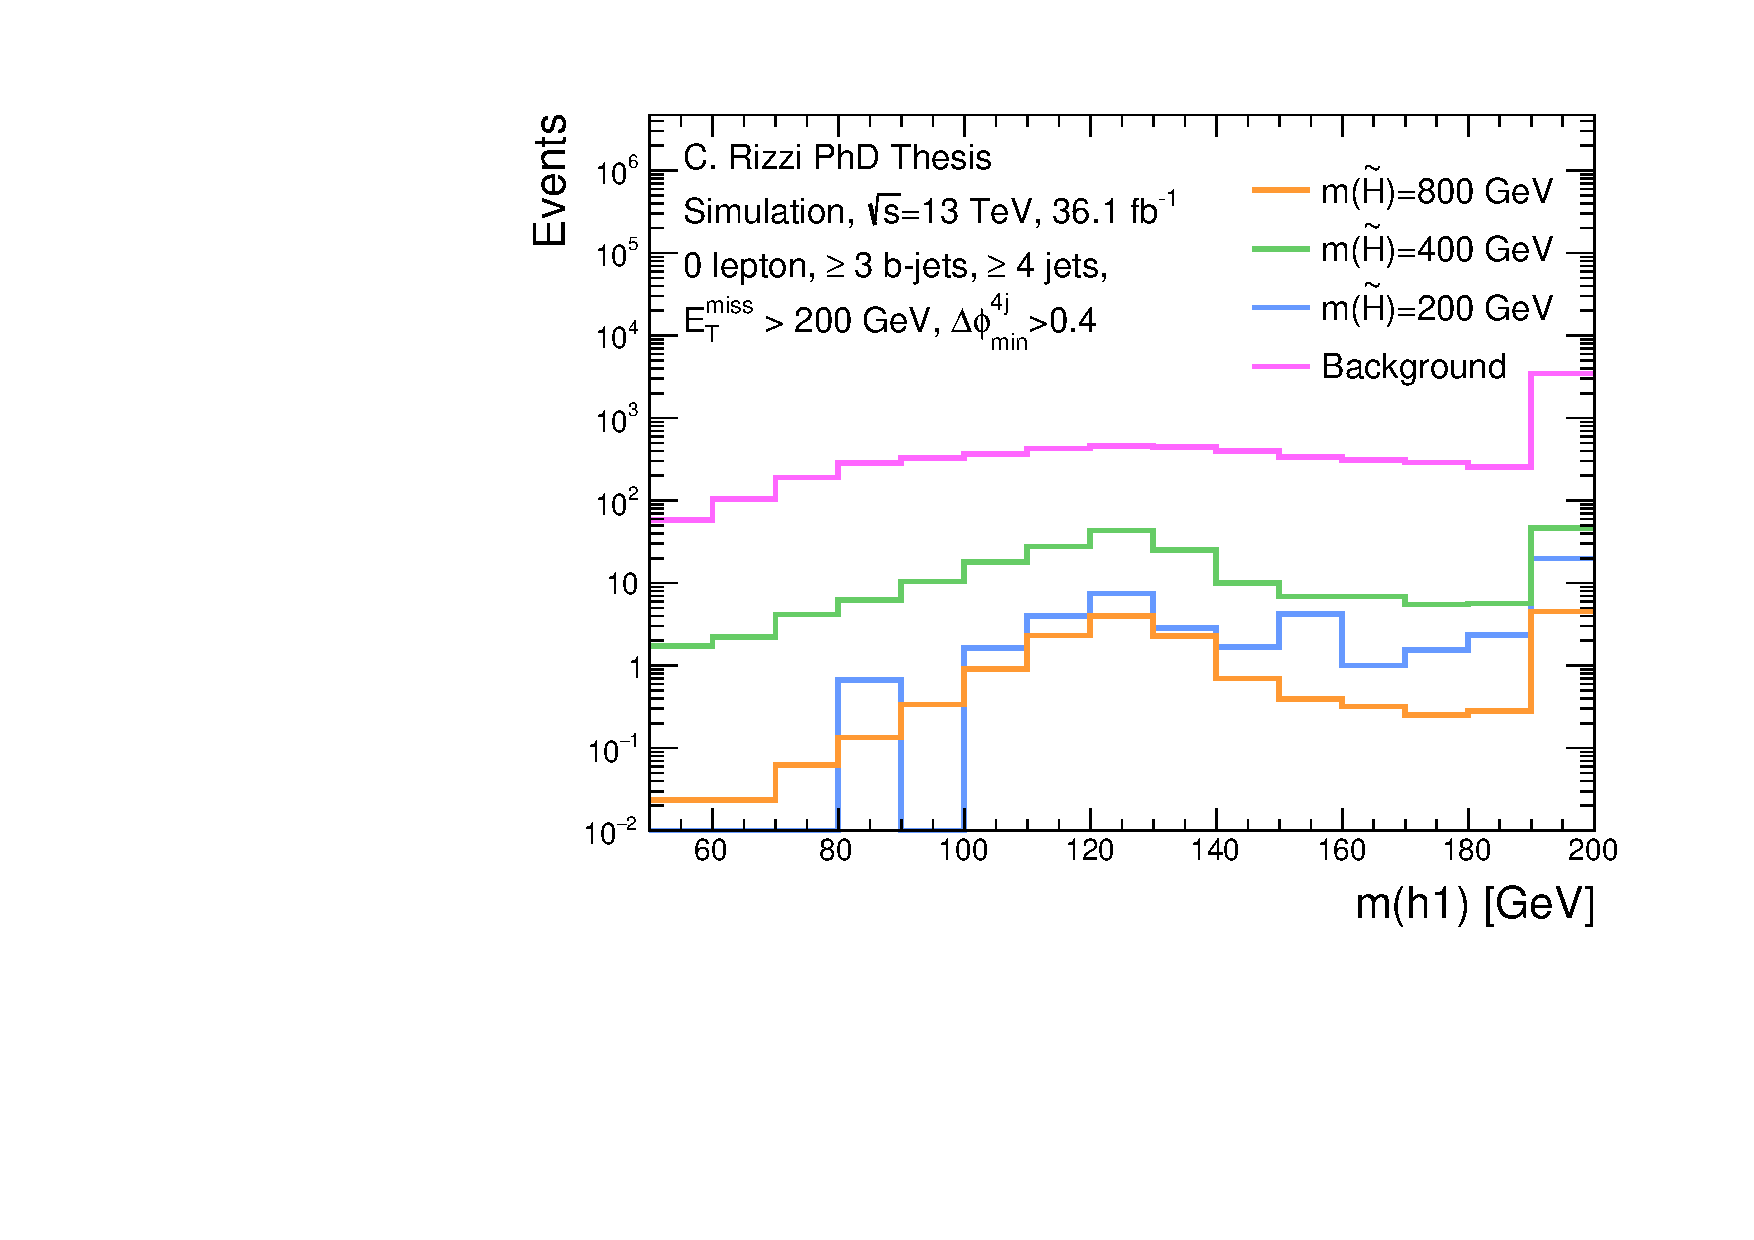
\includegraphics[width=0.325\textwidth]{figures/ewk_prod/sig_bkg/hh_compare_mass_h1_min_dR.pdf}\label{fig:ewk:sig:mass_h1_min_dR}}
\subfigure[m($h_2$)]{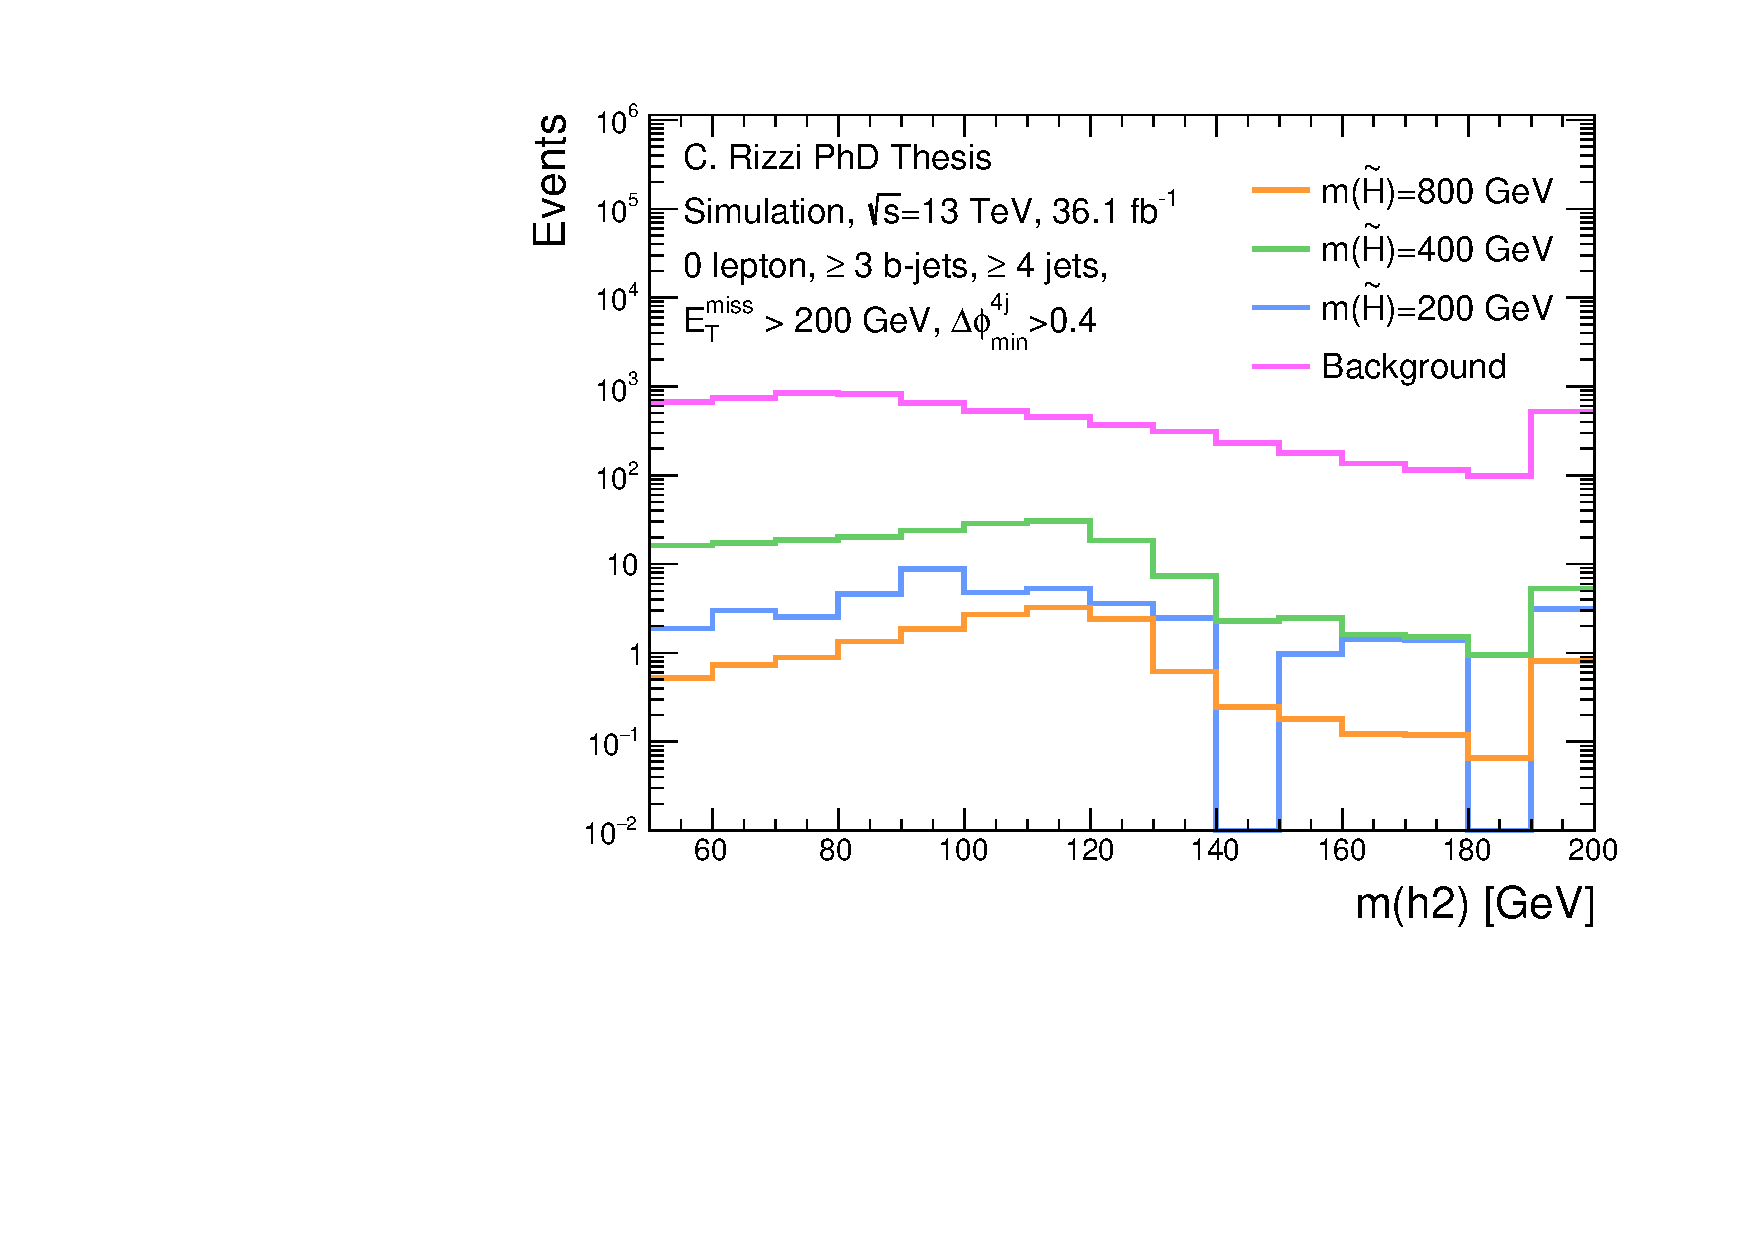
\includegraphics[width=0.325\textwidth]{figures/ewk_prod/sig_bkg/hh_compare_mass_h2_min_dR.pdf}\label{fig:ewk:sig:mass_h2_min_dR}}
\subfigure[\dRmax]{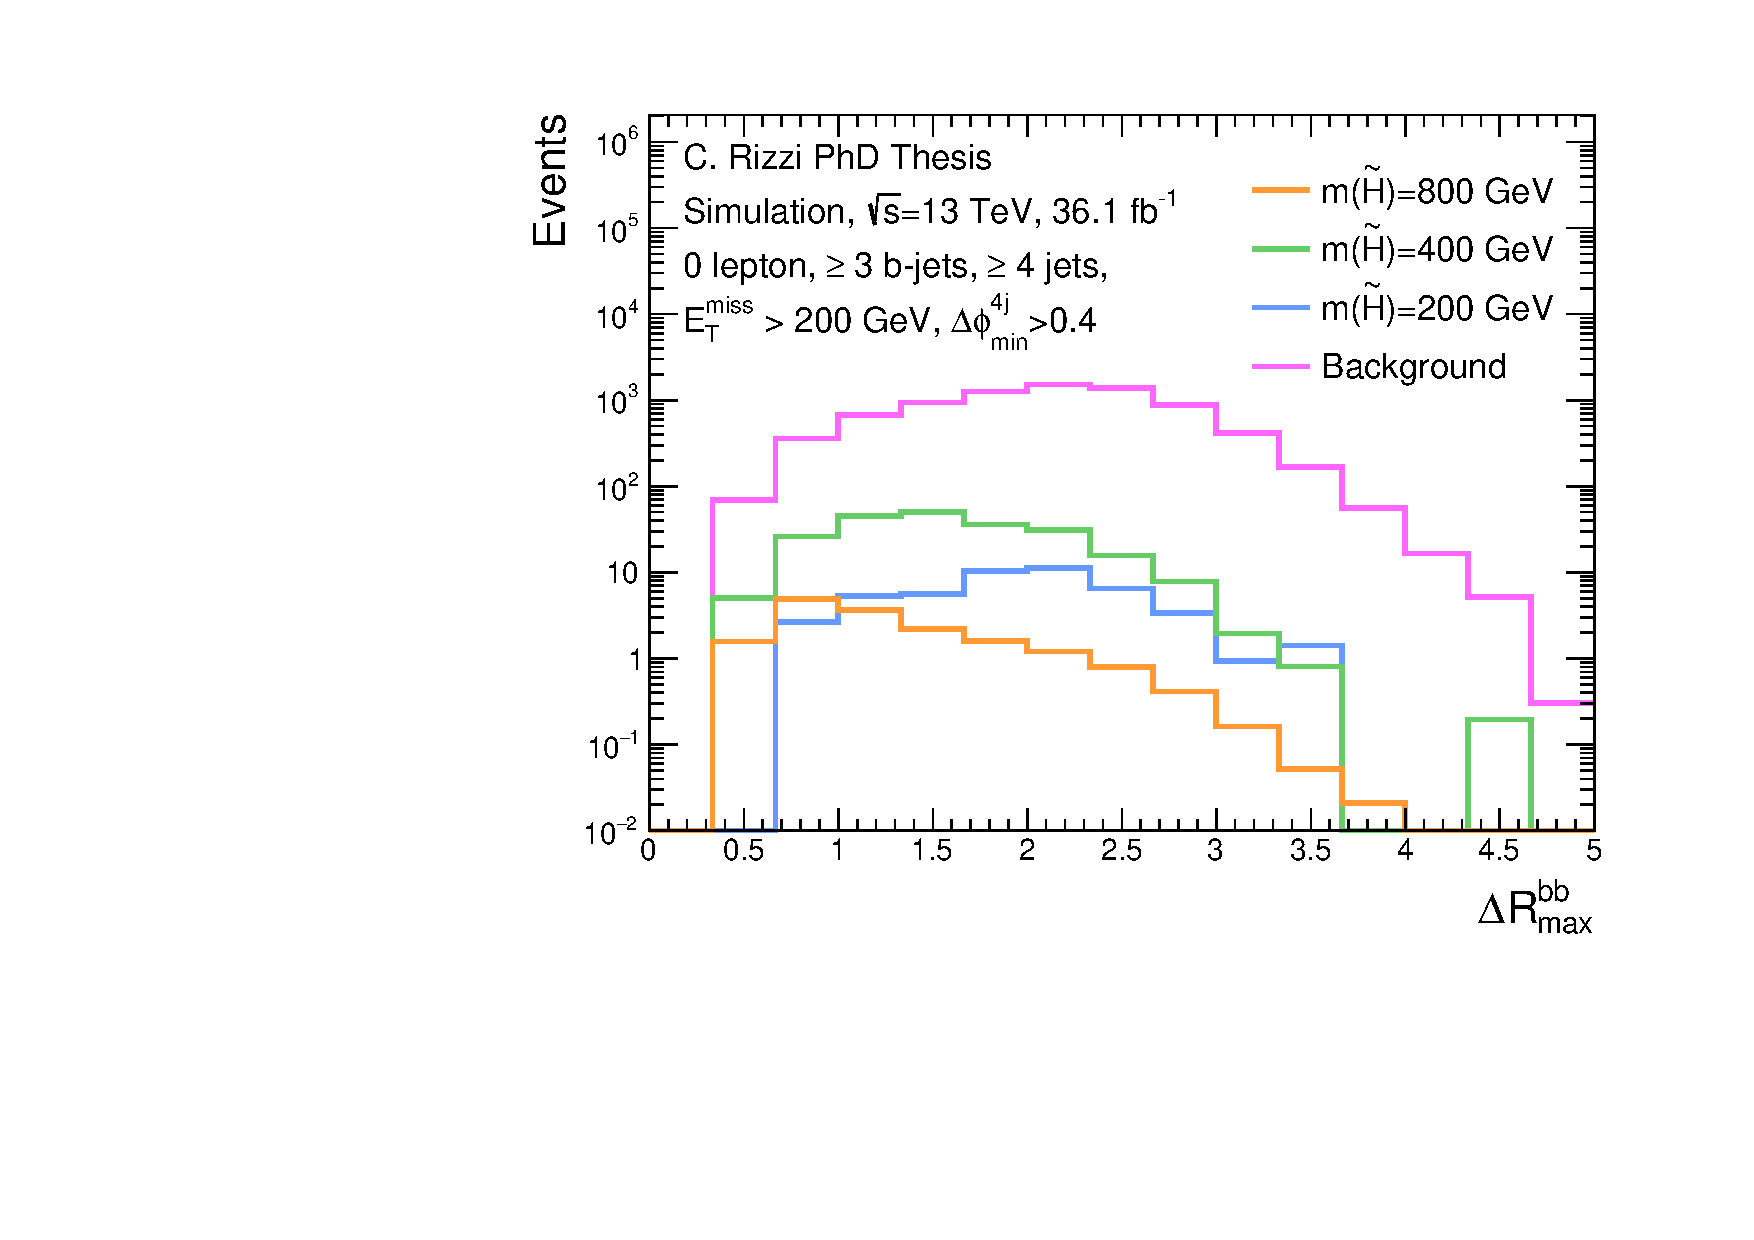
\includegraphics[width=0.325\textwidth]{figures/ewk_prod/sig_bkg/hh_compare_dRmax_dR.pdf}\label{fig:ewk:sig:dRmax_dR}}\\
\subfigure[\njet]{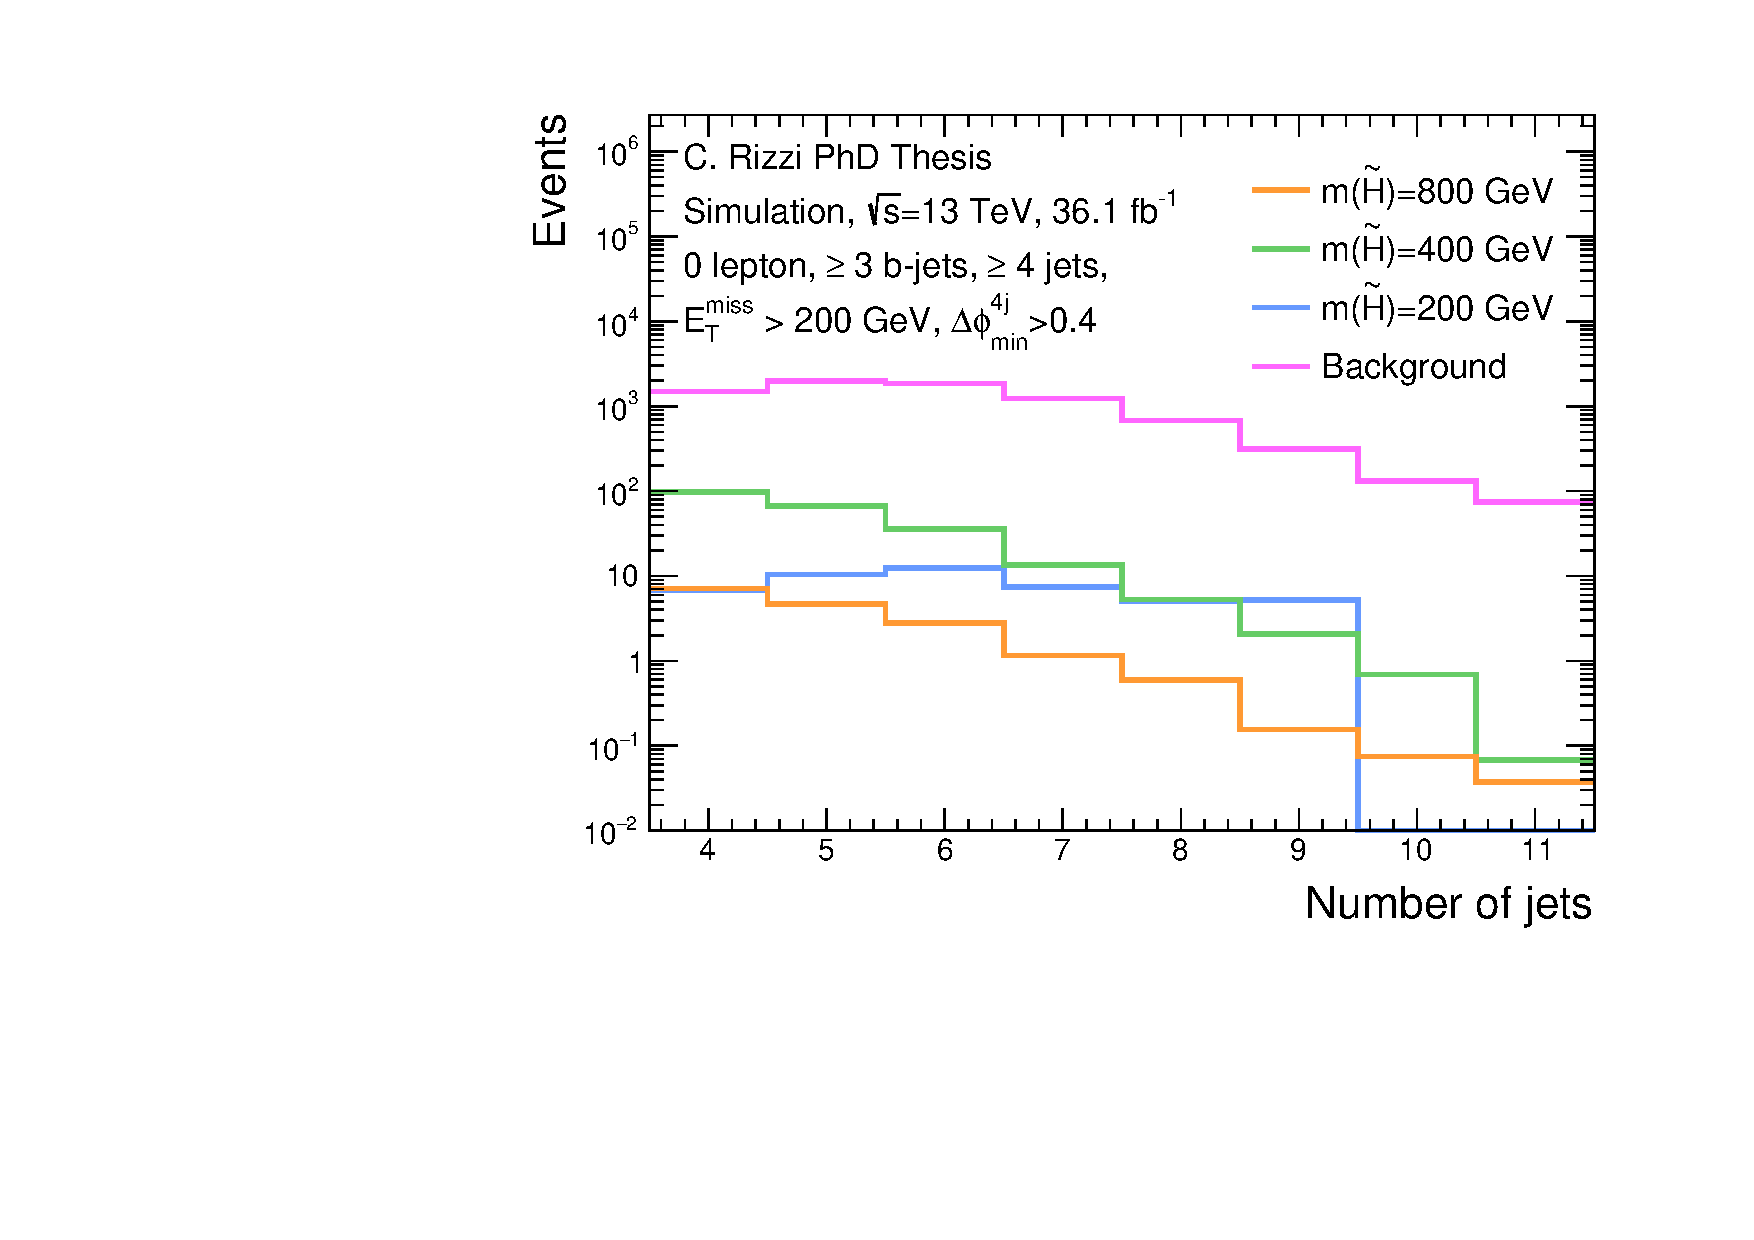
\includegraphics[width=0.325\textwidth]{figures/ewk_prod/sig_bkg/hh_compare_jets_n.pdf}\label{fig:ewk:sig:jets_n}}
\subfigure[\nbjet]{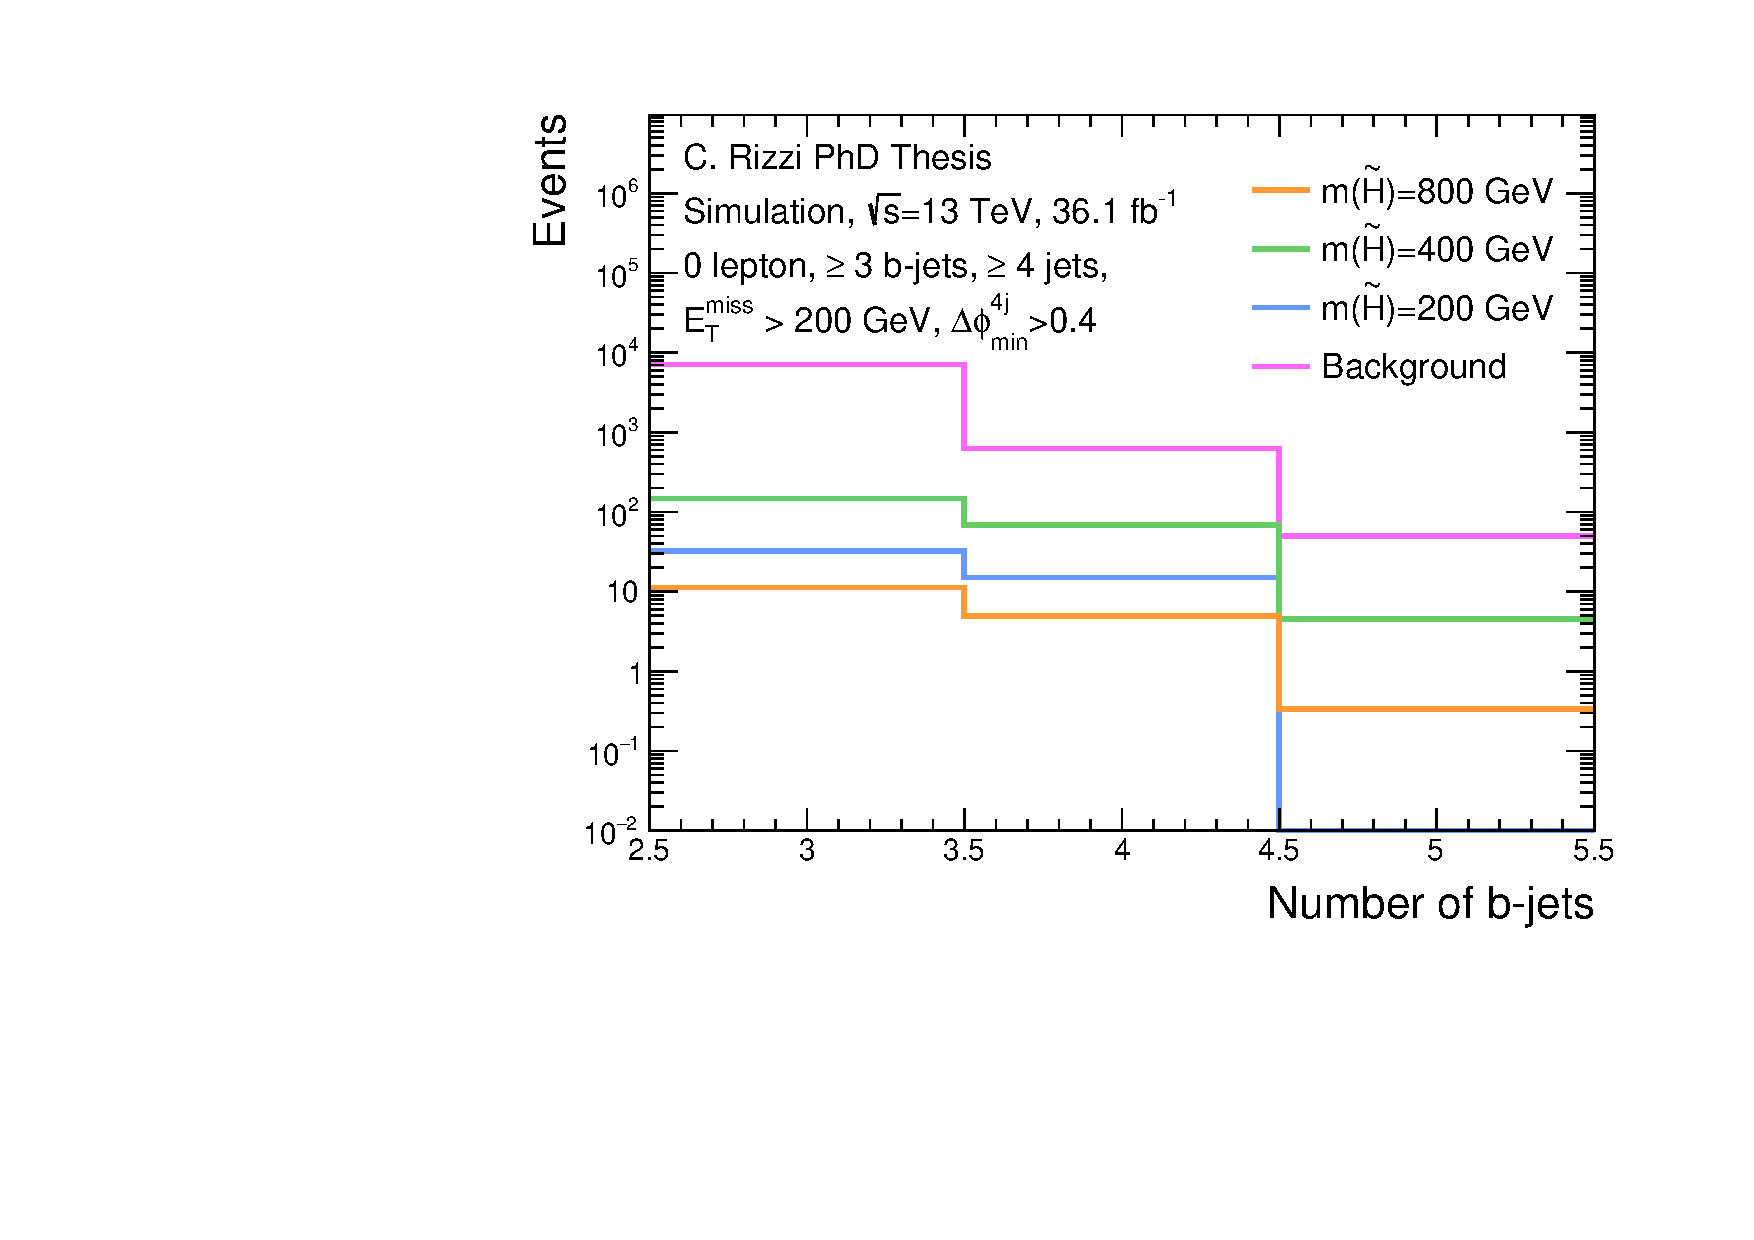
\includegraphics[width=0.325\textwidth]{figures/ewk_prod/sig_bkg/hh_compare_bjets_n.pdf}\label{fig:ewk:sig:bjets_n}}
\subfigure[\met]{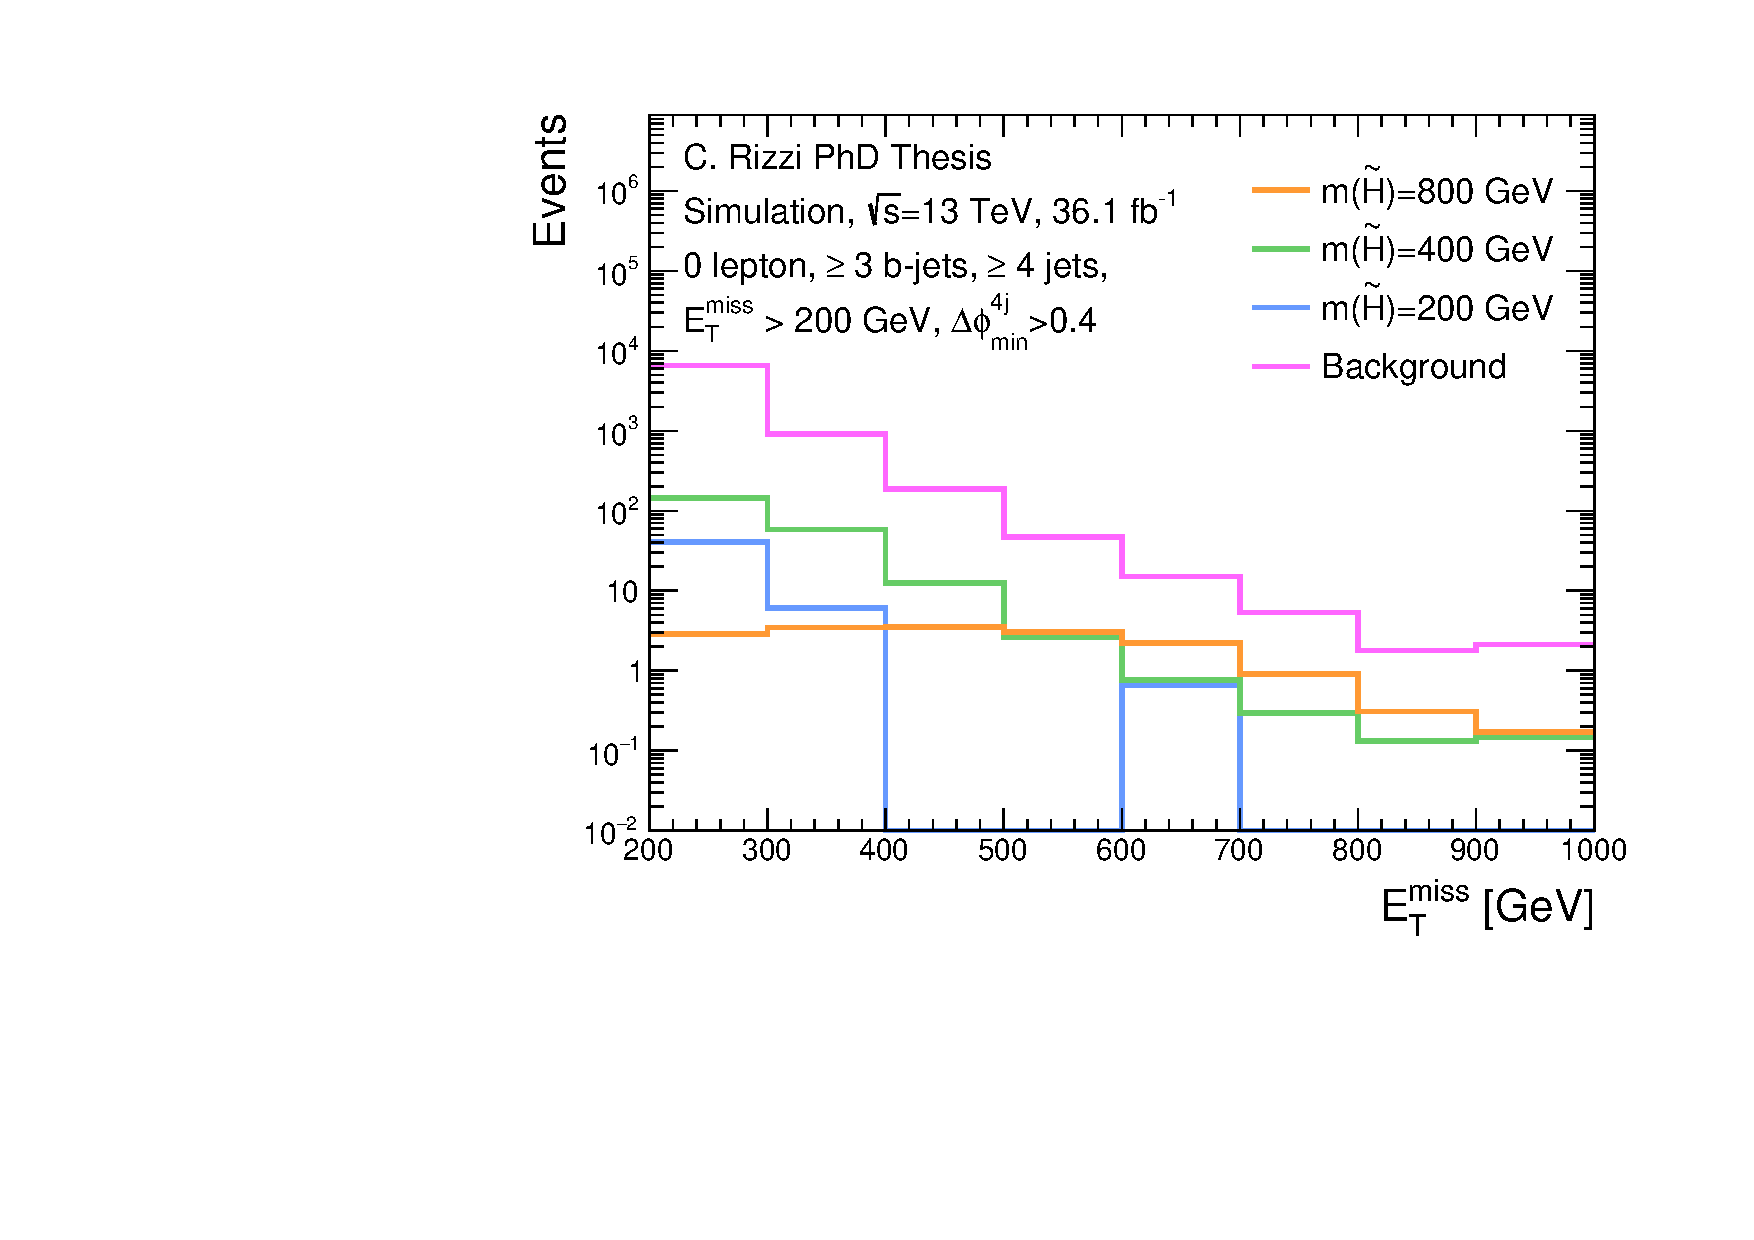
\includegraphics[width=0.325\textwidth]{figures/ewk_prod/sig_bkg/hh_compare_met.pdf}\label{fig:ewk:sig:met}}\\
\subfigure[\meffb]{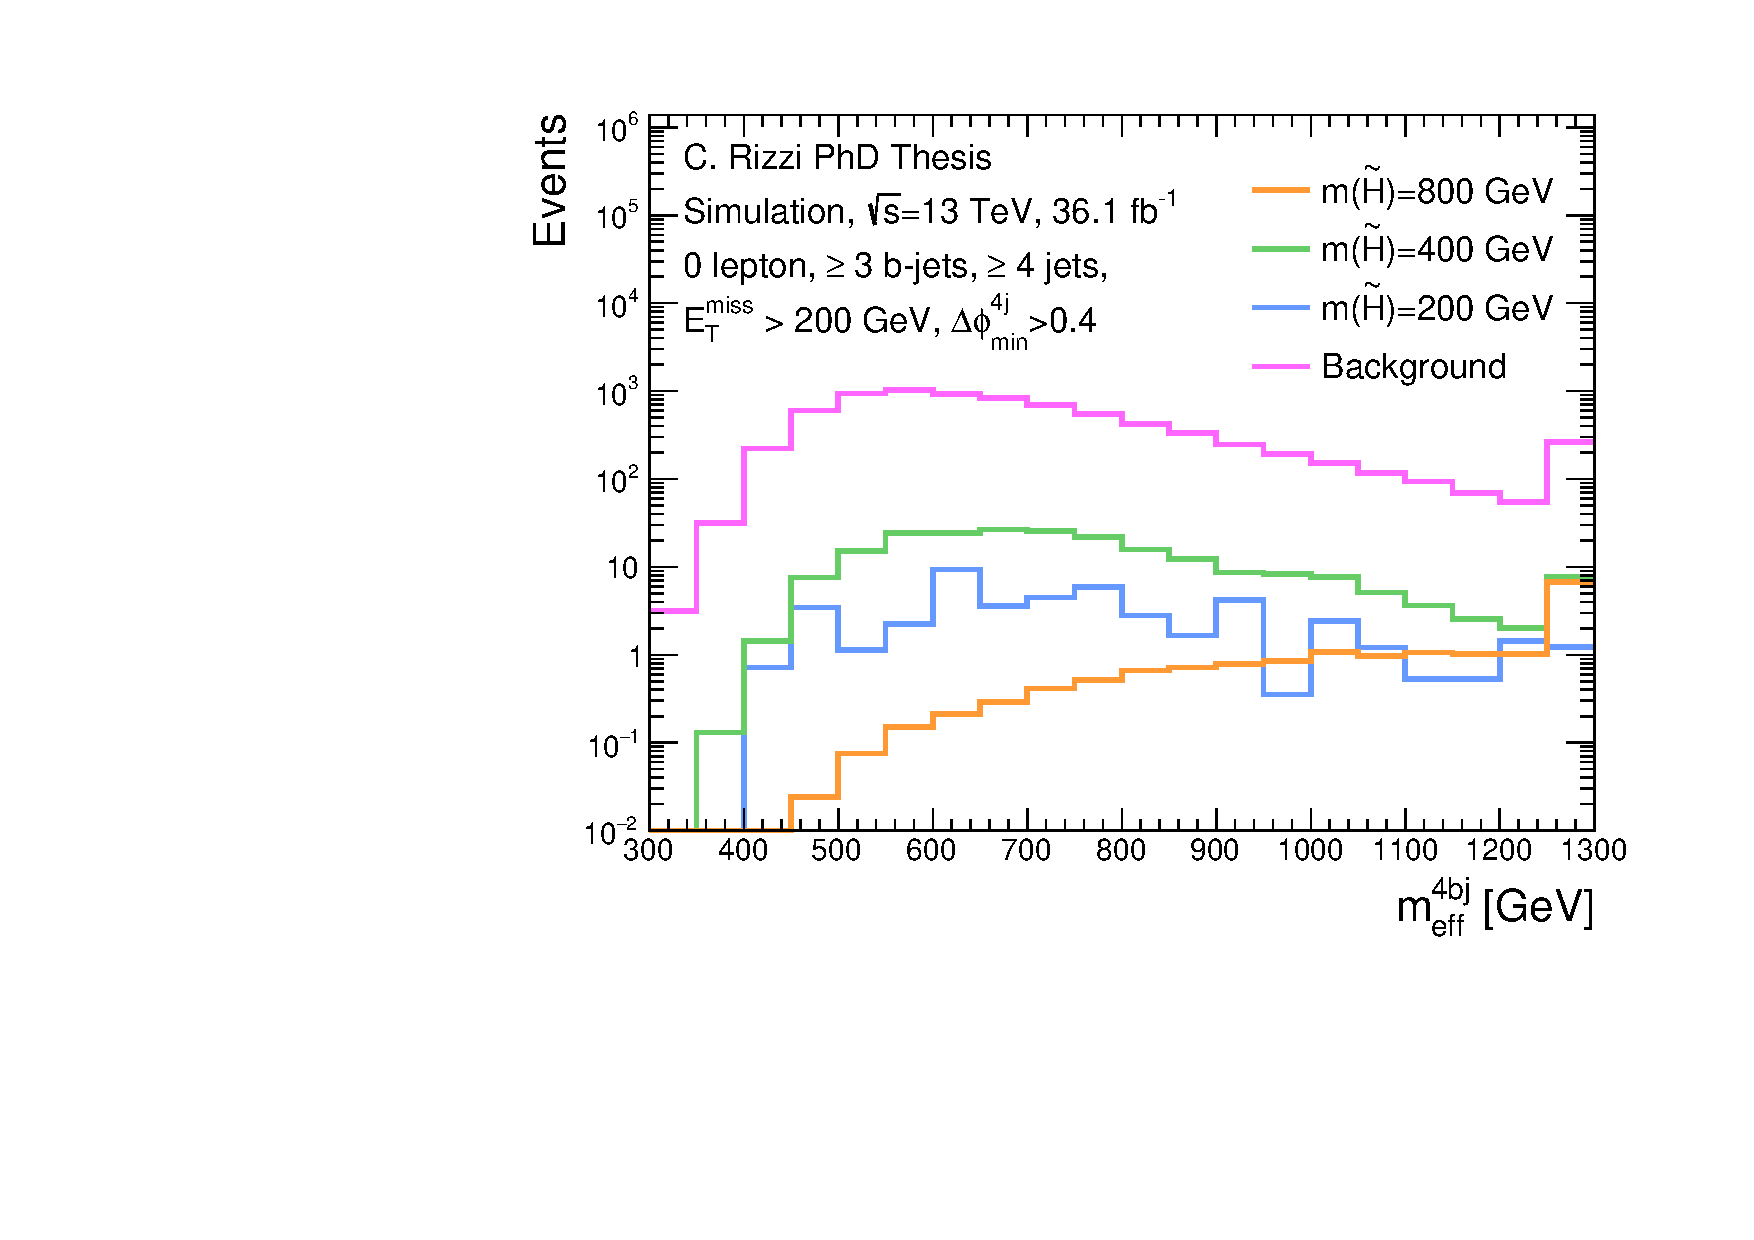
\includegraphics[width=0.325\textwidth]{figures/ewk_prod/sig_bkg/hh_compare_meff_4bj.pdf}\label{fig:ewk:sig:meff_4bj}}
\subfigure[\mtb]{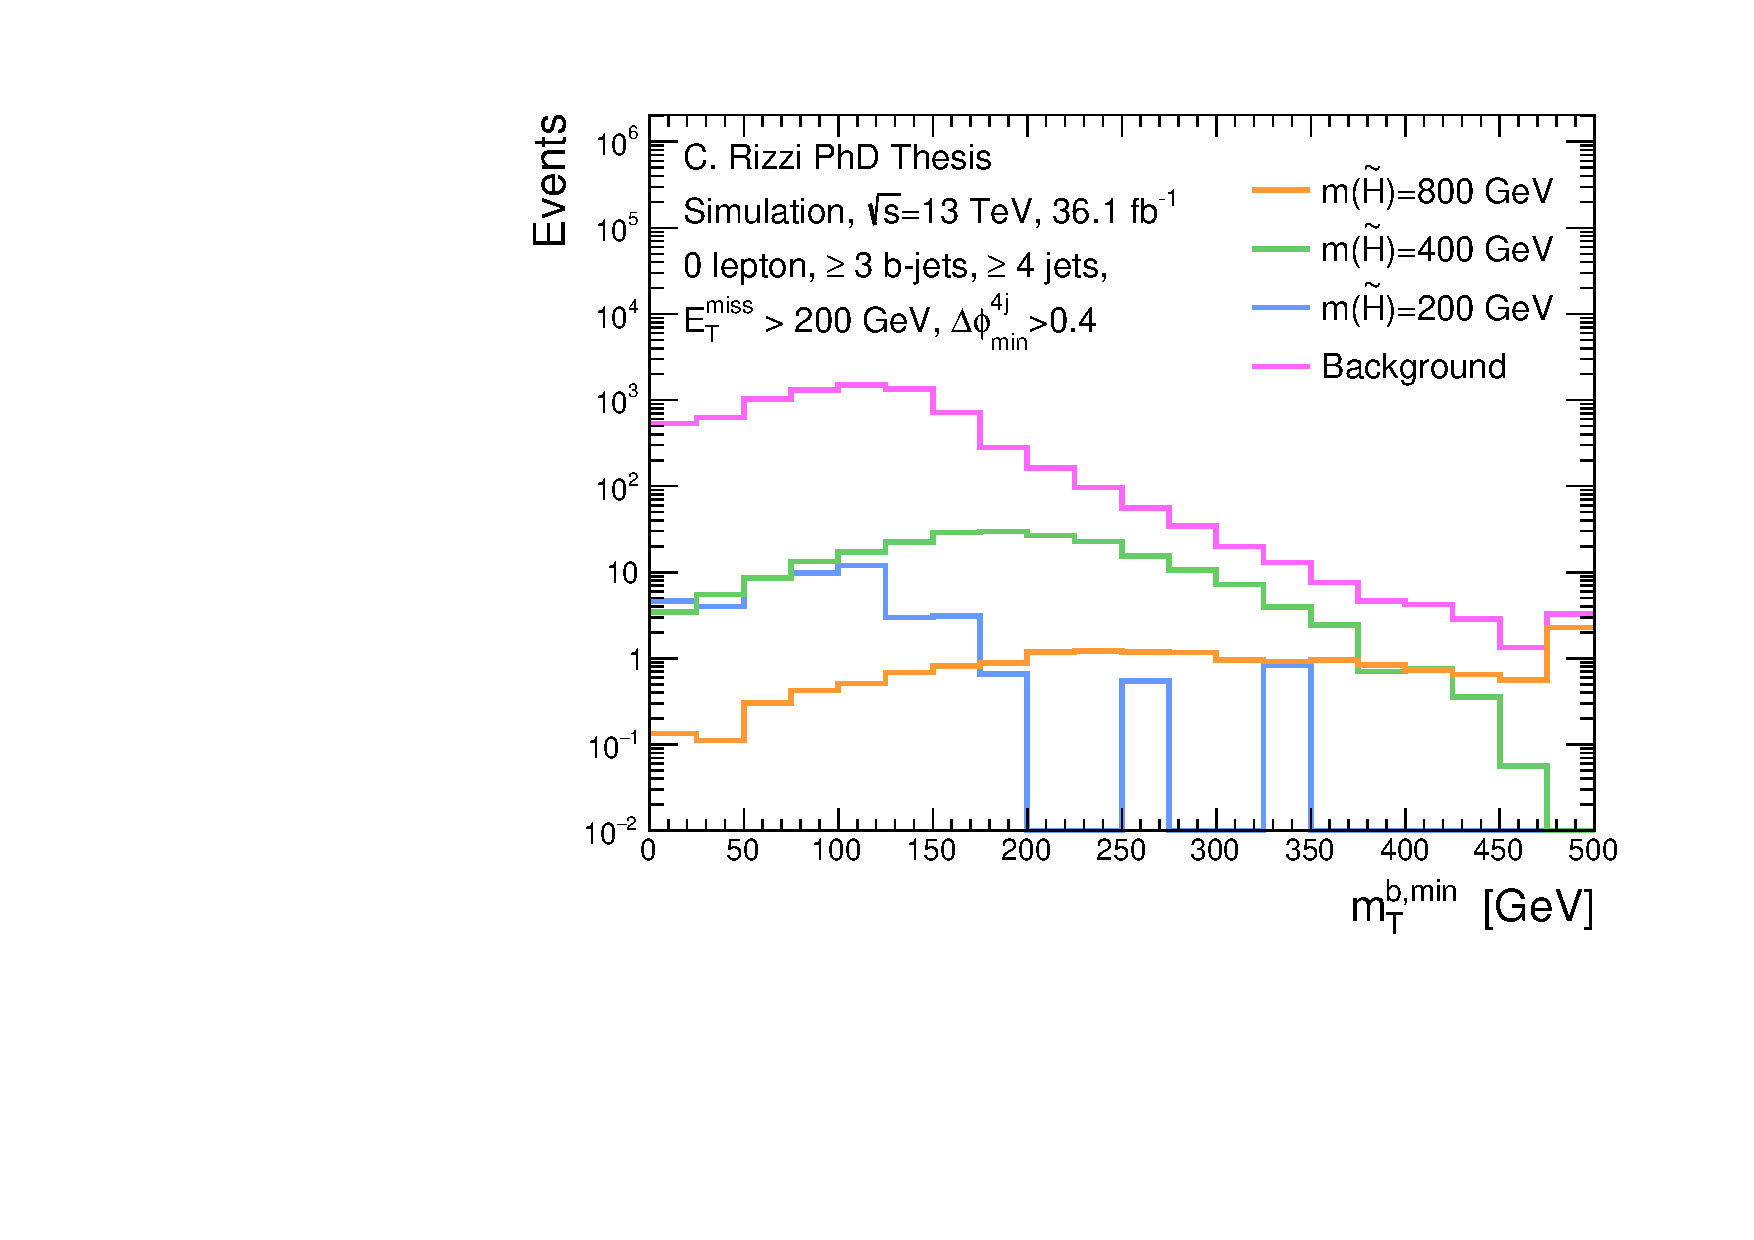
\includegraphics[width=0.325\textwidth]{figures/ewk_prod/sig_bkg/hh_compare_mTb_min.pdf}\label{fig:ewk:sig:mTb_min}}
\caption{Distribution of  the main kinematic variables in background and signal events after the selections described in the text.}
\label{fig:ewk:sig:1}
\end{figure*}

\FloatBarrier

\section{Signal regions}

This section describes the optimization of the \glspl{sr}. 
The high branching ratio of the h$\rightarrow$bb (58\%) makes the $\geq$3b channel the most promising to look for signal models 
in which both $\ninoone$ decay into h+$\gravino$. 
Therefore, the analysis selection are optimized to maximize the expected sensitivity to signals leading to $hh+\met$ 
and all the \glspl{sr} require both boson candidates to have masses compatible with the Higgs mass (the specific mass range is chosen during the optimization). 
%The target signal model is shown in Figure \ref{fig:opt_sighh4b}.

\begin{table}[htbp]
\begin{center}
%\resizebox{1.\textwidth}{!}{
\renewcommand{\arraystretch}{1.1}
\begin{tabular}{|l|c|c|c|}
\toprule
  & SR-3b-meff1-A & SR-3b-meff2-A & SR-3b-meff3-A\\
 \hline
\nbjet &  $=$3 &  $=$3 &  $\geq$3 \\
 \hline
\met & \multicolumn{3}{|c|}{$>$ 200}\\
\hline
\dphimin    & \multicolumn{3}{|c|}{$>$0.4}\\
 \hline
\njet &  4--5 &  4--5 &  4--5 \\
 \hline
\mtb &  $>$150 &  $>$150 &  $>$130 \\
 \hline
$m(h_1)$ &    \multicolumn{3}{|c|}{110--150}\\
 \hline
$m(h_2)$ &    \multicolumn{3}{|c|}{90--140}\\
 \hline
\dRmax &  0.4--1.4 &  0.4--1.4 &  0.4--1.4 \\
 \hline
\meffb &  600--850 &  850--1100 &  $>$1100  \\
\bottomrule
\end{tabular} 

\vspace{0.4cm}

\begin{tabular}{|l|c|c|c|c|c|}
\toprule
   & SR-4b-meff1-A & SR-4b-meff1-B & SR-4b-meff2-A & SR-4b-meff2-B  & SR-4b-meff1-A-disc \\
 \hline
\nbjet &  $\geq$4 &  $\geq$4 &  $\geq$4 &  $\geq$4  & $\geq4$\\
 \hline
\met & \multicolumn{5}{|c|}{$>$ 200}\\
\hline
\dphimin    & \multicolumn{5}{|c|}{$>$0.4}\\
 \hline
\njet & 4--5 &  4--5 &  4--6 &  4--6 & 4--5\\
 \hline
\mtb &   - & - & - & - & - \\
 \hline
$m(h_1)$ &    \multicolumn{5}{|c|}{110--150}\\
 \hline
$m(h_2)$ &    \multicolumn{5}{|c|}{90--140}\\
 \hline
\dRmax &   0.4--1.4 &  1.4--2.4 &  0.4--1.4 &  1.4--2.4 & 0.4--1.4 \\
 \hline
\meffb &  600--850 &  600--850 &  850--1100 &  850--1100 & $>600$ \\
\bottomrule
\end{tabular} 
%}
\caption{Signal region definitions for the high-mass analysis. The units of \met, \mtb, $m(h_1)$, $m(h_2)$, and \meffb are GeV. 
%These variables are defined in Section~\ref{high_event_selection}.
}
\label{tab:SR}
\end{center}
\end{table}

\section{Control and validation regions}

The \ttbar background is normalized in specifically designed \glspl{cr}.
A different \gls{cr} is built for each bin in \meffb and b-tagging multiplicity. 
These \glspl{cr} are built using side-bands both in m($h_1$) and m($h_2$). 
The extrapolation between \glspl{cr} and \glspl{sr} is tested in the \glspl{vr}, which take advantage of events
where only one between m($h_1$) and m($h_2$) is in the \gls{sr} mass range, 
as shown in Figure \ref{fig:binning_crvr}.

\begin{figure}[htbp]
	\centering
	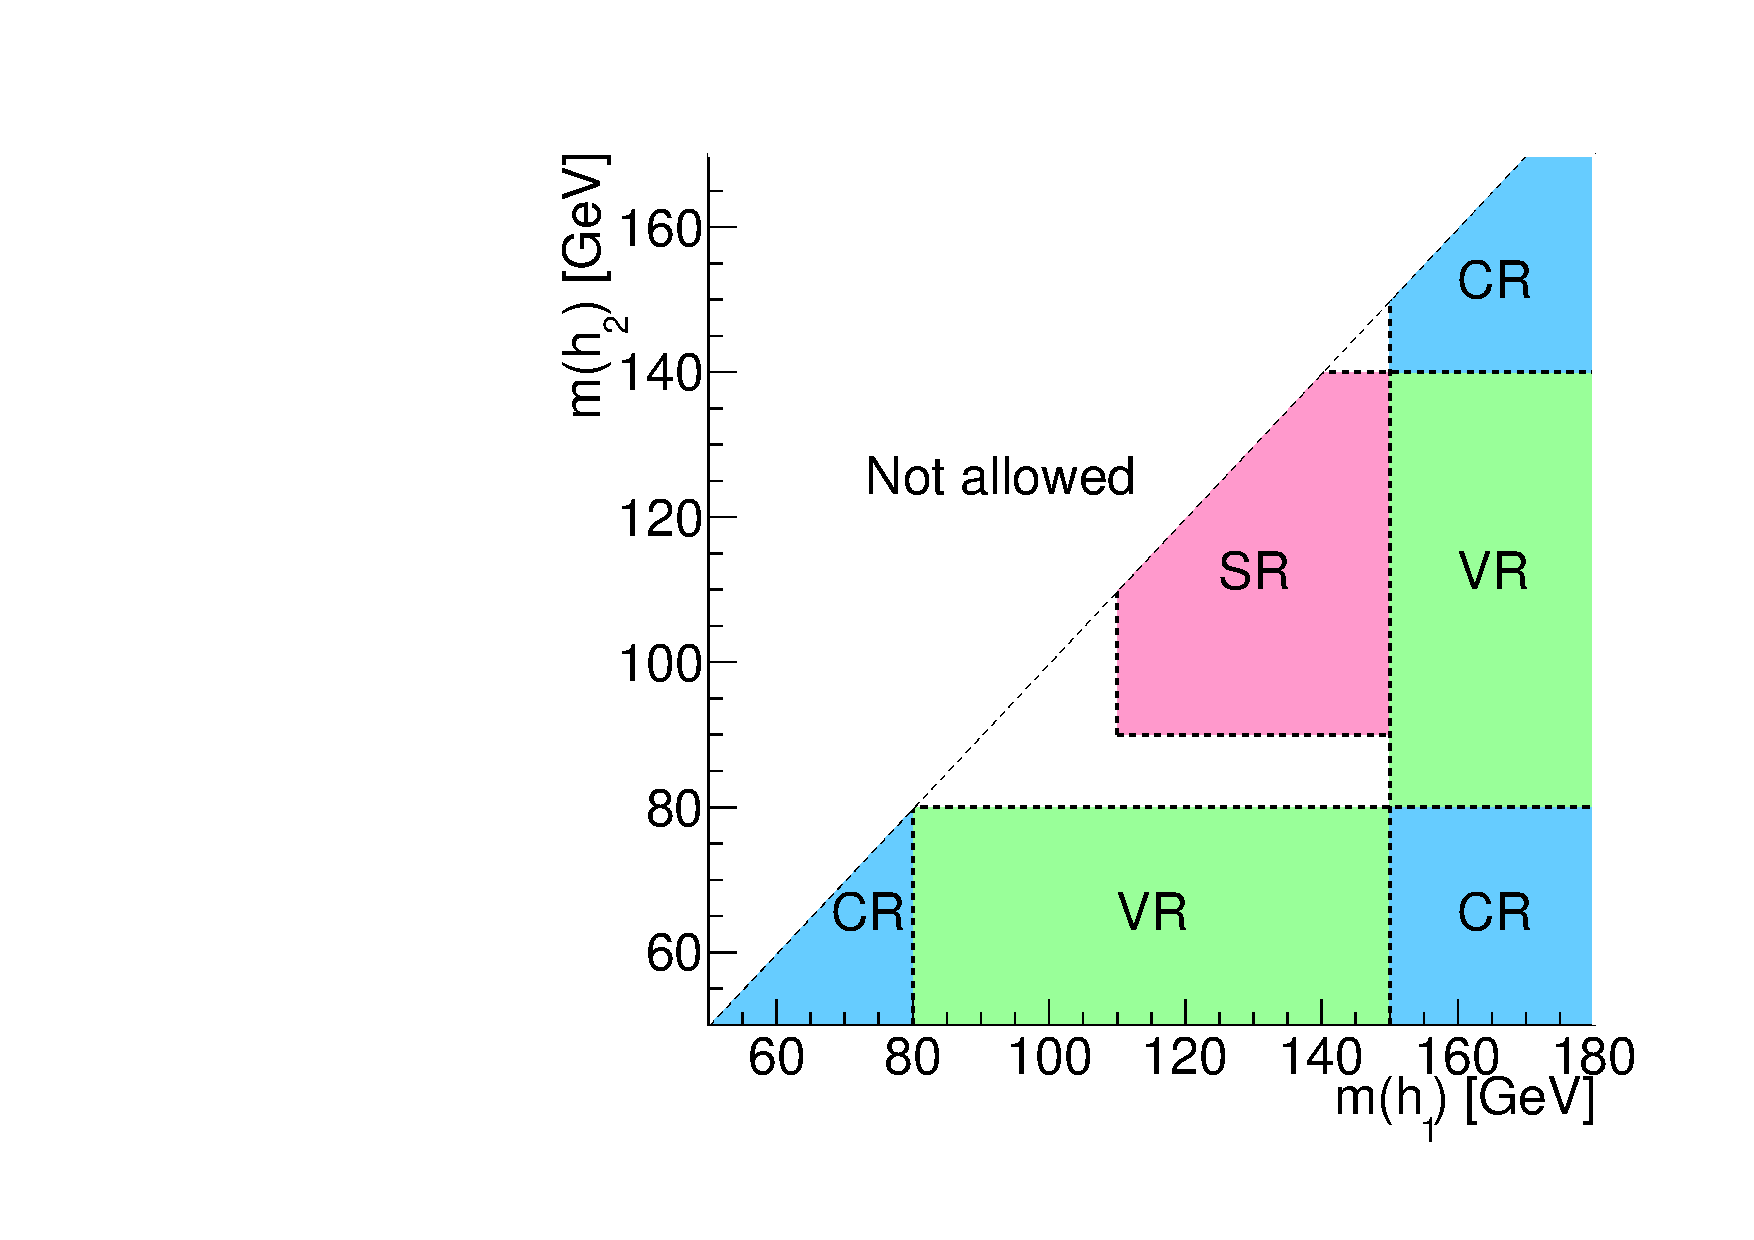
\includegraphics[width=0.490\textwidth]{figures/ewk_prod/varie/schema-1}
	\caption{The division of signal, control, and validation regions using the $m(h_1)$ and $m(h_2)$ variables in the high-mass analysis.}
	\label{fig:binning_crvr}
\end{figure}

Some of the selections of the \glspl{sr} are modified when moving to the \glspl{cr} or \glspl{vr}
 to allow enough statistics and low signal contamination.
The main extrapolation between \glspl{cr} and \glspl{sr} are:

\begin{itemize}
\item In the CR, both m($h_1$) and m($h_2$) are required to be outside the SR mass ranges.
\item \dRmax is relaxed to $<$4 (or removed).
\item \mtb is relaxed by 30 GeV in 3b-meff3 and by 50 GeV in 3b-meff1 and 3b-meff2.
\end{itemize}

To allow enough statistics in the VRs, the VRs are non orthogonal. Since these regions do not enter the fit, but are only used to validate the background prediction, non-orthogonality is not an issue here. 
The selections that remove the orthogonality between the different \glspl{vr} are:
\begin{itemize}
\item The edges of \meffb selection are relaxed by 50 GeV up and down.
\item The edges of the \dRmax bins are relaxed and, when two \dRmax bins are present for the same type of regions, they are partially overlapping.
\end{itemize}

With respect to the \glspl{sr}, the \mtb selection (where present) is relaxed as well by 50 GeV. 
Note that \glspl{cr} and \glspl{vr} do not have extrapolation in \nbjet or \njet with respect to the SRs.
The selections for all the \glspl{cr} and \glspl{vr} are summarized respectively in Tables \ref{tab:ewk:CR} and \ref{tab:ewk:VR}.


\begin{table}[htbp]
\begin{center}
%\resizebox{0.75\textwidth}{!}{
\renewcommand{\arraystretch}{1.1}
\begin{tabular}{|l|c|c|c|c|c|}
\toprule
  & CR-3b-meff1 & CR-3b-meff2 & CR-3b-meff3 & CR-4b-meff1 & CR-4b-meff2 \\
 \hline
\nbjet &  $=$3 &  $=$3 &  $\geq$3 &  $\geq$4 &  $\geq$4 \\
 \hline
\met  & \multicolumn{5}{|c|}{$>$ 200}\\
 \hline
\dphimin  & \multicolumn{5}{|c|}{$>$0.4}\\
 \hline
\njet &  4--5 &  4--5 &  4--5 &  4--5 &  4--6 \\
 \hline
\mtb &  $>$100 &  $>$100 &  $>$100 & - & - \\
 \hline
$m(h_1)$, $m(h_2)$  &  \multicolumn{5}{|c|}{ ($m(h_1)<$80, $m(h_2)<$80) or ($m(h_1)>$150, $m(h_2)<$80) or ($m(h_1)>$150, $m(h_2)>$140)    }\\
 \hline
\dRmax &  0.4--4 &  0.4--4 &  0.4--4 &  0.4--4 &  $\geq$ 0.4 \\
 \hline
\meffb &  600--850 &  850--1100 &  $>$1100 &  600--850 &  850--1100 \\
\bottomrule
\end{tabular} 
%} 
\caption{Control region definitions in the high-mass analysis. The units of \met, \mtb, $m(h_1)$, $m(h_2)$, and \meffb are GeV. 
%These variables are defined in Section~\ref{high_event_selection}.
}
\label{tab:ewk:CR}
\end{center}
\end{table}

\begin{table}[htbp]
\begin{center}
\renewcommand{\arraystretch}{1.1}
%\resizebox{1\textwidth}{!}{
\begin{tabular}{|l|c|c|c|}
\toprule
  & VR-3b-meff1-A & VR-3b-meff2-A & VR-3b-meff3-A \\
 \hline
\nbjet &  $=$3 &  $=$3 &  $\geq$3  \\
 \hline
\met  &  \multicolumn{3}{|c|}{$>$200}\\
 \hline
\dphimin &  \multicolumn{3}{|c|}{$>$0.4}\\
 \hline
\njet &  4--5 &  4--5 &  4--5 \\
 \hline
\mtb  & $>$120   & $>$100  & $>$80 \\
 \hline
$m(h_1)$, $m(h_2)$  &  \multicolumn{3}{|c|}{   (80<$m(h_1)$<150, $m(h_2)$<80) or ($m(h_1)$>150, 90<$m(h_2)$<140)   }\\
 \hline
\dRmax &  0.4--1.5 &  0.4--1.7 &  0.4--1.7  \\
 \hline
\meffb   & 550--900   & 800--1150  & $>$1050    \\
\bottomrule
\end{tabular} 

\vspace{0.4cm}

\begin{tabular}{|l|c|c|c|c|}
\toprule
  &  VR-4b-meff1-A & VR-4b-meff1-B & VR-4b-meff2-A & VR-4b-meff2-B \\
 \hline
\nbjet &   $\geq$4 &  $\geq$4 &  $\geq$4 &  $\geq$4 \\
 \hline
\met  &  \multicolumn{4}{|c|}{$>$200}\\
 \hline
\dphimin &  \multicolumn{4}{|c|}{$>$0.4}\\
 \hline
\njet &   4--5 &  4--5 &  4--6 &  4--6 \\
 \hline
\mtb   &  \multicolumn{4}{|c|}{-}\\
 \hline
$m(h_1)$, $m(h_2)$  &  \multicolumn{4}{|c|}{   (80<$m(h_1)$<150, $m(h_2)$<80) or ($m(h_1)$>150, 90<$m(h_2)$<140)   }\\
 \hline
\dRmax &   0.4--1.7 &  1.4--3 &  0.4--1.7 &  1.4--3 \\
 \hline
\meffb   &  550--900  & 550--900  & 800--1150  & 800--1150  \\
\bottomrule
\end{tabular} 
%} 
\caption{Validation region definitions in the high-mass analysis. The units of \met, \mtb, $m(h_1)$, $m(h_2)$, and \meffb are GeV. 
%These variables are defined in Section~\ref{high_event_selection}.
}
\label{tab:ewk:VR}
\end{center}
\end{table}

\section{Composition of the analysis regions}

\FloatBarrier

\section{Pre-fit Data-MC}

The modelling of the main kinematic variables is very similar to what observed in Section \ref{sec:strong:dataMC} 
for the strong-production multi-b analysis, as the few differences in object definitions are not enough to 
lead to a substantial change in data-\gls{mc} agreement; 
this section therefore focuses on the variables specific to Higgs boson reconstruction.
There is nevertheless a notable exception: in the analysis described in this chapter, the data-\gls{mc} agreement in the 
distribution of the number of b-jets is improved, as can be appreciated comparing Figure \ref{} with Figure \ref{}.
This is the result of the improvement in the b-tagging calibration, discussed in Section \ref{sec:obj:btaggingcalib}.
The other important difference with respect to the strong-production analysis is that in this case the analysis is performed 
only in regions with a lepton veto; it is not therefore sensitive to the mismodelling in the 1-lepton channel discussed in Section 
\ref{sec:strong:kinrw} and no kinematic reweighting is required. 


